% =============================================================
% 鸢尾花线性二分类示例：setosa 与其余类
% 编译方式：xelatex iris_linear_example.tex（两遍以生成目录）
% 角色：本 PDF 用于“解释代码及其运行过程”；可执行代码位于独立的
%       iris_linear_demo.py（不嵌入本文档）。
% 图形：优先 iris_boundary.png（脚本由 matplotlib 生成），
%       若不存在则退回 iris_figure.tex（脚本生成的 TikZ 片段）。
% =============================================================
\documentclass[UTF8, 11pt]{ctexart}

\usepackage{amsmath, amssymb}
\usepackage{graphicx}
\usepackage{booktabs}              % 三线表
\usepackage{geometry}
\geometry{margin=2.4cm, headheight=14pt}
\usepackage{enumitem}
\setlist{nosep}
\usepackage{caption}
\usepackage{xcolor}
\usepackage{pgfplots}
\pgfplotsset{compat=1.18}
\usepackage[colorlinks=true,
            linkcolor=blue!60!black,
            urlcolor=blue!60!black]{hyperref}

\title{\bfseries 鸢尾花线性二分类示例：setosa 与其余类}
\author{课程设计示例文档}
\date{2026 年 10 月}

% =============================================================
\begin{document}
\maketitle

\begin{abstract}
本文以真实的鸢尾花（Iris）数据集为例，仅使用前两个特征（萼片长、萼片宽），
将 setosa 与其余两类做二分类，并构建一个简单线性分类器（Fisher 线性判别，
闭式解）作为实际示例。全文聚焦“如何构建与解释一个线性分类器”，不做繁琐推导；
同时从结果出发，讨论其准确率、混淆矩阵与结论边界。
\end{abstract}

\tableofcontents
\newpage

% ============================================================
\section{引言与背景}
\label{sec:intro}

分类是监督学习的核心任务之一。在《Python机器学习：原理与实践》的方法论主线中，
模型复杂度由\textbf{线性模型}起步，逐步过渡到决策树、集成学习，直至支持向量机
（SVM）及其核方法。线性方法因其可解释性强、具有闭式解，是理解更复杂模型的
最佳起点。

本文的目标是：以一个真实数据集为对象，演示如何\textbf{构建}一个线性分类器、
如何\textbf{解释}其决策边界，并如何\textbf{评估}其泛化能力。为此我们刻意选择
一个接近线性可分的子问题——鸢尾花的 setosa 与其余两类在前两个特征下的二分类，
使线性方法的边界形态得以直观呈现。

% ============================================================
\section{数据来源与预处理}
\label{sec:data}

数据取自 \textbf{UCI Machine Learning Repository} 的 Iris 数据集
（R.~A.~Fisher, 1936），可从
\url{https://archive.ics.uci.edu/dataset/53/iris} 获取；
亦可经由 scikit-learn 内置函数 \verb|load_iris()| 载入
（二者同源，数值一致）。本文示例读取本地文件 \verb|iris.data|。

该数据集共 $n=150$ 个样本、3 个类别（各 50 个），每条记录含 4 个特征与 1 个类别标签。
本示例仅保留前两个特征：
\begin{itemize}
  \item $x_1$：萼片长度（sepal length，单位 cm）；
  \item $x_2$：萼片宽度（sepal width，单位 cm）。
\end{itemize}
并将标签重编码为二值：\textbf{setosa 记为 $y=1$}（正类），其余两类合并记为 $y=0$（负类）。

% ============================================================
\section{模型与方法：Fisher 线性判别}
\label{sec:model}

本例采用 \textbf{Fisher 线性判别（LDA）}——一种线性方法，具有闭式解，无需迭代优化。
其判别函数为
\begin{equation}
  g(\mathbf{x}) = \mathbf{w}^{\mathsf{T}}\mathbf{x} + b,
  \qquad
  \hat{y} = \begin{cases}
    1 & (g(\mathbf{x}) > 0),\\[2pt]
    0 & (\text{否则}),
  \end{cases}
  \label{eq:g}
\end{equation}
其中 $\mathbf{x}=(x_1,x_2)^{\mathsf{T}}$。判别方向 $\mathbf{w}$ 与偏置 $b$ 由训练数据闭式给出：
\begin{align}
  \mathbf{w} &= \mathbf{S}_w^{-1}(\boldsymbol{\mu}_1 - \boldsymbol{\mu}_0),\label{eq:w}\\
  b &= -\mathbf{w}^{\mathsf{T}}\!\left(\frac{\boldsymbol{\mu}_1+\boldsymbol{\mu}_0}{2}\right),\label{eq:b}
\end{align}
这里 $\boldsymbol{\mu}_1,\boldsymbol{\mu}_0$ 分别为两类样本均值，$\mathbf{S}_w$ 为
\textbf{类内散布矩阵}：
\begin{equation}
  \mathbf{S}_w = \sum_{k\in\{0,1\}}\;
                 \sum_{\mathbf{x}_i \in C_k}
                 (\mathbf{x}_i - \boldsymbol{\mu}_k)(\mathbf{x}_i - \boldsymbol{\mu}_k)^{\mathsf{T}}.
  \label{eq:sw}
\end{equation}
决策边界即 $\mathbf{w}^{\mathsf{T}}\mathbf{x}+b=0$，是一条\textbf{直线}（线性），
这正是“线性方法”的含义；式~\eqref{eq:w} 中 $\mathbf{S}_w^{-1}$ 在代码中以
\texttt{numpy.linalg.solve} 求解并加微小正则，数值更稳定。

% ============================================================
\section{实验设置}
\label{sec:setup}
\begin{itemize}
  \item \textbf{特征}：第 1、2 列（萼片长、萼片宽），未做标准化；
  \item \textbf{标签}：setosa $\to y=1$，其余 $\to y=0$；
  \item \textbf{划分}：按 $7:3$ 切分训练/测试集（训练 105、测试 45），
        固定随机种子（\verb|default_rng(42)|，等价于 \verb|random_state=42|）保证可复现；
  \item \textbf{拟合}：仅用训练集估计 $\boldsymbol{\mu}_1,\boldsymbol{\mu}_0,\mathbf{S}_w$，
        再作用于测试集（避免数据泄露）。
\end{itemize}

% ============================================================
\section{结果与分析}
\label{sec:results}

\subsection{判别参数与决策边界}
由训练集估计得到的线性分类器参数为
\[
  \mathbf{w} = \begin{pmatrix} -0.0672 \\ 0.1163 \end{pmatrix},
  \qquad b = 0.0150.
\]
决策边界方程为
\[
  -0.0672\,x_1 + 0.1163\,x_2 + 0.0150 = 0,
  \quad\text{即}\quad
  x_2 \approx 0.5774\,x_1 - 0.1291.
\]
该直线将特征平面划分为“判为 setosa”（$g>0$）与“判为其余类”（$g\le 0$）两个区域。

\subsection{准确率与混淆矩阵}

\begin{table}[htbp]
  \centering
  \caption{关键数值（一次确定性运行结果）}
  \label{tab:res}
  \begin{tabular}{l r}
    \toprule
    项目 & 数值 \\
    \midrule
    样本总数 $n$ & 150 \\
    setosa ($y=1$) / 其余 ($y=0$) & 50 / 100 \\
    训练 / 测试样本 & 105 / 45 \\
    $w_1$（萼片长系数） & $-0.0672$ \\
    $w_2$（萼片宽系数） & $0.1163$ \\
    截距 $b$ & $0.0150$ \\
    训练准确率 & $98.10\%$ \\
    测试准确率 & $97.78\%$ \\
    \bottomrule
  \end{tabular}
\end{table}

\begin{table}[htbp]
  \centering
  \caption{混淆矩阵（行=真实，列=预测）}
  \label{tab:cm}
  \begin{tabular}{l cc cc}
    \toprule
    & \multicolumn{2}{c}{训练集} & \multicolumn{2}{c}{测试集} \\
    \cmidrule(lr){2-3} \cmidrule(lr){4-5}
    真实 $\backslash$ 预测 & 负类 & 正类 & 负类 & 正类 \\
    \midrule
    负类（其余） & 72 & 2 & 26 & 0 \\
    正类（setosa） & 0 & 31 & 1 & 18 \\
    \bottomrule
  \end{tabular}
\end{table}

图~\ref{fig:boundary} 给出两类样本散点与所学决策边界。可见 setosa 在
“小萼片长、大萼片宽”区域聚集，被一条直线较好分开。

\begin{figure}[htbp]
  \centering
  \IfFileExists{iris_boundary.png}{%
    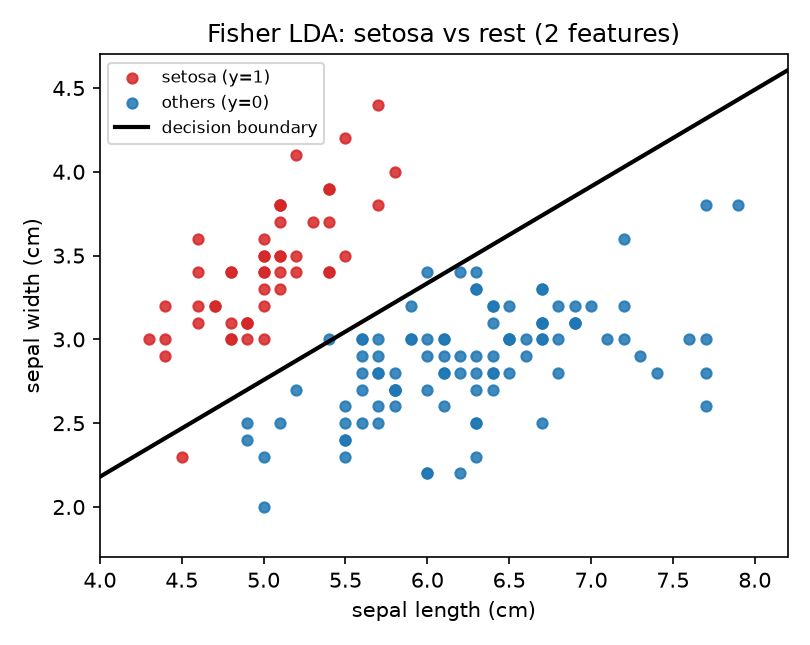
\includegraphics[width=9cm]{iris_boundary.png}%
  }{%
    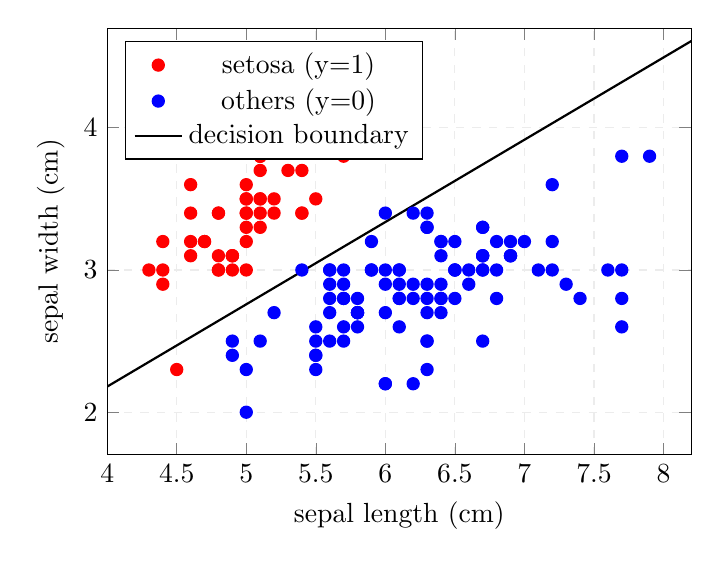
\begin{tikzpicture}
\begin{axis}[
  width=9cm, height=7cm,
  xlabel={sepal length (cm)}, ylabel={sepal width (cm)},
  xmin=4.00, xmax=8.20, ymin=1.70, ymax=4.70,
  legend pos=north west, grid=major, grid style={lightgray!30, dashed},
  tick label style=/pgf/number format/fixed
]
  \addplot[only marks, mark=*, red, mark size=2.2pt] coordinates { (5.10,3.50) (4.90,3.00) (4.70,3.20) (4.60,3.10) (5.00,3.60) (5.40,3.90) (4.60,3.40) (5.00,3.40) (4.40,2.90) (4.90,3.10) (5.40,3.70) (4.80,3.40) (4.80,3.00) (4.30,3.00) (5.80,4.00) (5.70,4.40) (5.40,3.90) (5.10,3.50) (5.70,3.80) (5.10,3.80) (5.40,3.40) (5.10,3.70) (4.60,3.60) (5.10,3.30) (4.80,3.40) (5.00,3.00) (5.00,3.40) (5.20,3.50) (5.20,3.40) (4.70,3.20) (4.80,3.10) (5.40,3.40) (5.20,4.10) (5.50,4.20) (4.90,3.10) (5.00,3.20) (5.50,3.50) (4.90,3.10) (4.40,3.00) (5.10,3.40) (5.00,3.50) (4.50,2.30) (4.40,3.20) (5.00,3.50) (5.10,3.80) (4.80,3.00) (5.10,3.80) (4.60,3.20) (5.30,3.70) (5.00,3.30) };
  \addplot[only marks, mark=*, blue, mark size=2.2pt] coordinates { (7.00,3.20) (6.40,3.20) (6.90,3.10) (5.50,2.30) (6.50,2.80) (5.70,2.80) (6.30,3.30) (4.90,2.40) (6.60,2.90) (5.20,2.70) (5.00,2.00) (5.90,3.00) (6.00,2.20) (6.10,2.90) (5.60,2.90) (6.70,3.10) (5.60,3.00) (5.80,2.70) (6.20,2.20) (5.60,2.50) (5.90,3.20) (6.10,2.80) (6.30,2.50) (6.10,2.80) (6.40,2.90) (6.60,3.00) (6.80,2.80) (6.70,3.00) (6.00,2.90) (5.70,2.60) (5.50,2.40) (5.50,2.40) (5.80,2.70) (6.00,2.70) (5.40,3.00) (6.00,3.40) (6.70,3.10) (6.30,2.30) (5.60,3.00) (5.50,2.50) (5.50,2.60) (6.10,3.00) (5.80,2.60) (5.00,2.30) (5.60,2.70) (5.70,3.00) (5.70,2.90) (6.20,2.90) (5.10,2.50) (5.70,2.80) (6.30,3.30) (5.80,2.70) (7.10,3.00) (6.30,2.90) (6.50,3.00) (7.60,3.00) (4.90,2.50) (7.30,2.90) (6.70,2.50) (7.20,3.60) (6.50,3.20) (6.40,2.70) (6.80,3.00) (5.70,2.50) (5.80,2.80) (6.40,3.20) (6.50,3.00) (7.70,3.80) (7.70,2.60) (6.00,2.20) (6.90,3.20) (5.60,2.80) (7.70,2.80) (6.30,2.70) (6.70,3.30) (7.20,3.20) (6.20,2.80) (6.10,3.00) (6.40,2.80) (7.20,3.00) (7.40,2.80) (7.90,3.80) (6.40,2.80) (6.30,2.80) (6.10,2.60) (7.70,3.00) (6.30,3.40) (6.40,3.10) (6.00,3.00) (6.90,3.10) (6.70,3.10) (6.90,3.10) (5.80,2.70) (6.80,3.20) (6.70,3.30) (6.70,3.00) (6.30,2.50) (6.50,3.00) (6.20,3.40) (5.90,3.00) };
  \addplot[no marks, thick, black] coordinates { (4.00,2.18) (8.20,4.61) };
  \legend{setosa (y=1), others (y=0), decision boundary}
\end{axis}
\end{tikzpicture}
%
  }
  \caption{setosa 与其余类在前两个特征上的散点及线性决策边界
    （图形由 \texttt{iris\_linear\_demo.py} 生成：有 matplotlib 时为 PNG，否则为 TikZ）。}
  \label{fig:boundary}
\end{figure}

\subsection{分析与讨论}
\begin{itemize}
  \item \textbf{泛化表现稳健}：训练准确率 $98.10\%$ 与测试准确率 $97.78\%$ 之差仅约
        $0.32$ 个百分点，未出现过拟合，模型在训练集与测试集上表现一致。
  \item \textbf{误分样本集中在边界附近}：由表~\ref{tab:cm}，训练集有 2 个负类被误判为
        正类（FP），测试集有 1 个正类被漏判（FN），合计 150 个样本中仅 3 个误分；
        这正是“近似线性可分”的直观体现——少数点跨越了决策边界。
  \item \textbf{印证奥卡姆剃刀}：仅用两维特征与一个线性分类器即取得约 $98\%$ 准确率，
        说明该子问题无需更复杂模型，简单方法已足够。
  \item \textbf{结论边界}：高准确率来自“两维下 setosa 可较好分离”的数据特性，
        而非模型复杂；当数据呈明显非线性边界时，应转向核方法（教材第 8 章 SVM）。
\end{itemize}

% ============================================================
\section{结论}
\label{sec:conclusion}

在该二分类任务上，简单的线性分类器即取得约 $98\%$ 的准确率，说明仅用
“萼片长、萼片宽”两维已能较好区分 setosa 与其余类。但准确率并非 $100\%$，
且混淆矩阵显示存在少量跨边界样本，表明 setosa 在这两个特征上“近似”而非
“完全”线性可分——这是数据本身的特性，并不等于线性模型“万能”。本示例完整呈现了
“数据 $\to$ 模型 $\to$ 评估 $\to$ 解释”的线性分类流程，可作为更复杂模型（如
第 8 章支持向量机及其核方法）的对照基线。

% ============================================================
\section{读者需确认的关键事项清单}
\label{sec:checklist}
\begin{enumerate}
  \item \textbf{数据来源与版本}：数据来自 UCI Iris（Fisher, 1936），
        与 \verb|sklearn.load_iris()| 同源；若改用 \verb|load_iris()|，
        请确认其返回的特征顺序与标签编码一致（前两列为萼片长、萼片宽）。
  \item \textbf{标签定义}：正类设为 setosa（$y=1$），其余两类合并为 $y=0$；
        若交换定义，判别系数符号整体取反，但决策边界不变。
  \item \textbf{特征与单位}：仅使用第 1、2 列（萼片长、萼片宽，单位 cm），
        未做标准化；本例近似可分故可行，换用其他数据须谨慎。
  \item \textbf{可复现性}：训练/测试划分由固定随机种子
        （\verb|default_rng(42)|）决定；更换种子，准确率会有小幅波动，结论不变。
  \item \textbf{线性可分性}：setosa 与前两维下的其余类“近似”而非“完全”
        线性可分（故准确率 $\approx 98\%$ 而非 $100\%$），这是数据特性。
  \item \textbf{模型假设}：本例采用 Fisher 线性判别（LDA，闭式解），属线性方法；
        若数据非线性可分，应改用核方法或更复杂模型（教材第 8 章 SVM）。
  \item \textbf{结论边界}：高准确率来自“两维下 setosa 可较好分离”，
        并非模型复杂；本示例意在演示线性分类器的构建与边界，而非追求性能上限。
  \item \textbf{依赖与运行}：可执行代码 \texttt{iris\_linear\_demo.py} 仅需
        Python~3 + NumPy，无需 scikit-learn；图形优先用 matplotlib 生成 PNG，
        否则退回 TikZ 片段。本文档（PDF）仅作解释用途，编译需同目录的
        图形文件（\texttt{iris\_boundary.png} 或 \texttt{iris\_figure.tex}）。
\end{enumerate}

% ============================================================
\appendix
\section{代码说明与运行}
\label{sec:code}
本文档仅用于\textbf{解释代码及其运行过程}；可执行代码位于独立的
\texttt{iris\_linear\_demo.py}，并不嵌入本文档。相关文件如下：

\begin{itemize}
  \item \texttt{iris\_linear\_demo.py}：主程序（仅依赖 NumPy；绘图可选 matplotlib）。
  \item \texttt{iris.data}：UCI Iris 原始数据（本地副本，亦可由 \texttt{sklearn.load\_iris()} 获取）。
  \item \texttt{iris\_linear\_results.txt}：脚本运行后生成的“说明 + 数值 + 混淆矩阵”文本。
  \item \texttt{iris\_boundary.png} 或 \texttt{iris\_figure.tex}：决策边界图（二选一，由脚本生成）。
\end{itemize}

\paragraph{运行方式}
在终端执行 \verb|python iris_linear_demo.py|（需 Python~3 与 NumPy）。
若环境中已安装 Matplotlib，脚本额外输出 \texttt{iris\_boundary.png}；
否则自动退化为输出 TikZ 片段 \texttt{iris\_figure.tex}，供本文档绘图使用。
绘图失败不影响核心数值产出（结果仍写入 txt）。

\paragraph{脚本流程}
\begin{enumerate}
  \item 读取本地 \texttt{iris.data}，仅取前两特征（萼片长、萼片宽），并将 setosa 标为 $y=1$、其余类标为 $y=0$；
  \item 以固定随机种子（\verb|default_rng(42)|）按 $7:3$ 划分训练/测试集；
  \item 仅用训练集，按 Fisher 线性判别（LDA）闭式解估计 $\mathbf{w}, b$（式~\eqref{eq:w}--\eqref{eq:b}）；
  \item 在训练集与测试集上评估准确率与混淆矩阵；
  \item 将说明文字与全部数值写入 \texttt{iris\_linear\_results.txt}，并尝试绘制决策边界。
\end{enumerate}

\paragraph{与本文档的关系}
本文档的“数据来源 / 模型 / 结果与分析 / 结论 / 清单”等章节，正是对上述代码所实现方法及其
运行结果（表~\ref{tab:res}、表~\ref{tab:cm}、图~\ref{fig:boundary}）的解释。
代码本身可独立运行，不依赖 LaTeX。

% ============================================================
\begin{thebibliography}{9}
\bibitem{fisher36} R.~A.~Fisher. The use of multiple measurements in taxonomic
  problems. \emph{Annals of Eugenics}, 7(2):179--188, 1936.
\bibitem{uci} UCI Machine Learning Repository. \emph{Iris Data Set}.
  \url{https://archive.ics.uci.edu/dataset/53/iris}.
\bibitem{sklearn} scikit-learn developers. \verb|sklearn.datasets.load_iris|.
  \url{https://scikit-learn.org/}.
\bibitem{book} 《Python机器学习：原理与实践》第 8 章，支持向量机（线性方法与核方法的延伸参照）.
\end{thebibliography}

\end{document}
